\documentclass[11pt]{article}
\usepackage{graphics,epsfig,amsmath,amssymb}
\usepackage{epsf}
\usepackage{boxedminipage}
\usepackage{fullpage}
\usepackage{fancyheadings}
\usepackage{times}
\usepackage{amsmath}
\usepackage{ifthen}
\usepackage{pseudocode}
\usepackage{psfrag}
\pagestyle{fancy}

\setlength{\topmargin}{.2in}
\setlength{\parindent}{0in}
\setlength{\parskip}{.15in}
\setlength{\footskip}{0.1in}

\newcounter{pctr}
\stepcounter{pctr}

\newcounter{partctr}

\newcommand{\ie}{{\em i.e.}}
\newcommand{\eg}{{\em e.g.}}

\newcommand{\ch}{\item {\bf True~~/~~False~~}}
\newcommand{\tfnote}{\probnote{Circle True or False for each choice.}}
\newcommand{\allapply}{\probnote{Circle ALL that apply}}
\newcommand{\bestanswer}{\probnote{Circle the BEST answer}}
\newcommand{\ansbelow}{\probnote{Answer legibly in the space below.}}

\renewcommand{\thesection}{{\bf\Roman{section}}}
\renewcommand{\theenumi}{{\bf\Alph{enumi}.}}
\renewcommand{\labelenumi}{{\bf\Alph{enumi}.}}

\newcommand{\setversion}[1]{\def\version{#1}}
\setversion{quiz}

\ifthenelse{\equal{\version}{answers}}{
    \newcommand{\sols}[1]{#1}
} {
    \newcommand{\sols}[1]{}
}


\newcounter{answer}
\newenvironment{answer}[1][\relax]{\refstepcounter{answer}\begin{list}%
 {}{\leftmargin 0pt\rightmargin 0pt\labelsep 3pt\parsep 0pt%
 \setlength{\listparindent}{\parindent}}
    \item {\bf Answer \theanswer #1}\
    }{\hspace*{\fill}$\blacksquare$\end{list}} 



% uses these macros to delimit problems
\newcommand\prob[1]%
  {\begin{itemize}\item[]%
   \vspace{.2in}{\bf\thepctr. ~[#1~ points]:}\stepcounter{pctr}}
\newcommand\eprob{\end{itemize}}
\newcommand\probnote[1]%
  {\\\begin{tabular}{cr} \hspace{3in} & {\bf (#1)} \\ \end{tabular}}

% headers/footers
\lhead[\fancyplain{}{\bf Page \thepage ~of \pageref{lastpage}}]%
      {CS 3251 Spring 2013, Quiz 2}
\lfoot[{\bf Initials: }]%
      {{\bf Initials: }}
\rhead[CS 3251 Spring 2013, Quiz 2]%
      {\fancyplain{}{\bf Page \thepage ~of \pageref{lastpage}}}
\cfoot{}
\setlength{\headrulewidth}{0in}
\setlength{\headsep}{.3in}

 % Compact itemize and enumerate.  Note that they use the same counters and
% symbols as the usual itemize and enumerate environments.
\def\compactify{\itemsep=0pt \topsep=0pt \partopsep=0pt \parsep=0pt}
\let\latexusecounter=\usecounter
\newenvironment{CompactItemize}
  {\def\usecounter{\compactify\latexusecounter}
   \begin{itemize}}
  {\end{itemize}\let\usecounter=\latexusecounter}
\newenvironment{CompactEnumerate}
  {\def\usecounter{\compactify\latexusecounter}
   \begin{enumerate}}
  {\end{enumerate}\let\usecounter=\latexusecounter}

\begin{document}
\cfoot{}
\pagestyle{empty}
\begin{center}
\begin{tabular}{lr}
\resizebox{1in}{!}{
\includegraphics{GT}}
&
\parbox{4in}{
    {\Large\it College of Computing} \\ \\
    {\LARGE\sf Georgia Institute of Technology} 
}
%
\end{tabular}
\end{center}

\begin{center}
{\Large{\bf CS 3251: Computer Networking: Spring 2013} \\
 \vspace{.15in} \Huge{\bf Quiz II}} 
\vspace{.2in}

% this is the box on the first page with overall quiz information
\begin{boxedminipage}[h]{6in}
There are \underline{12 questions} and \underline{\pageref{lastpage}
  pages} in this quiz booklet (including this page), plus one optional
bonus question. {\bf There are 90 total points.}  Answer each question according to the instructions
given.  You have {\bf 85 minutes} to answer the questions.

\vspace{.1in} The last page is an easy, optional set of questions.  {\em
  Rip this page off of your exam for five bonus points.}  Turn it in
anonymously.


\vspace{.1in} 
If you find a question ambiguous, write down any
assumptions you make.  {\bf Be neat and legible.}  If I can't
understand your answer, I can't give you credit!  
%There are three pretty
%challenging questions (clearly marked); you may want to look through the
%whole quiz and save those for last.

\vspace{.1in} 
Use the empty sides of this booklet if you need scratch space.  You
may also use them for answers, although you shouldn't need to.  {\em If you
do use the blank sides for answers, make sure to clearly say so!}

\vspace{.1in} 
{\bf Note well: Write your name in the space below AND your initials at the bottom of each
page of this booklet.}

\begin{center}{\bf THIS IS AN ``CLOSED BOOK'' QUIZ.\\
NO BOOKS, NO NOTES, NO OTHER MATERIALS, NO PHONES, NO COMPUTERS, NO
LAPTOPS, NO PDAS.\\ 
ONE TWO-SIDED LETTER-SIZED NOTE SHEET IS ALLOWED.
%NO ENCRYPTED WIRELESS TRAFFIC. \\
MAKE SURE YOU'VE READ ALL THE INSTRUCTIONS ABOVE!}
\end{center}
{\em Initial here to indicate that (1)~you've read the instructions and (2)~
you agree to abide by the Georgia Tech Honor Code: }



\if 0
\vspace{.05in} The last page has easy bonus questions, {\em which you can
answer outside of the allotted time}.  Rip the last page off of your
quiz for five bonus points.  Turn it in anonymously if you like (feel
free to fill it out after the quiz and give it to a TA, or take it with you).  You
won't get the five points if you don't tear off the page (this is to
make certain you've read this far ;).
\fi 

\end{boxedminipage}
\end{center}
\begin{center}
{\it Do not write in the boxes below}
\end{center}
\begin{center}
\begin{tabular}{|l|l|l|l|l|l|l|l|l|} \hline \hline
{\bf 1-5 (xx/20)}& {\bf 6-8 (xx/18)} & {\bf 9-10 (xx/21)} & {\bf 11-13
  (xx/23)} & {\bf 14 (xx/8)} &{\bf Bonus (xx+5/10)} & {\bf Total
  (xx/90)}  \\ \hline 
 & & & & & & \\ 
 & & & & & & \\ \hline \hline
\end{tabular}
\end{center}

\vspace{.05in}
{\bf\Large{Name:}}

\newpage
\pagestyle{fancy}

\section{Warmup}



\prob{4} 
Which of the following is true about content distribution networks?
\allapply
\setcounter{partctr}{0}
\begin{list}{\bf\Alph{partctr}.}{\usecounter{partctr}}
\item Content distribution networks can improve the
  performance that a client sees by reducing the network latency between
  the client and the content that it is downloading.
\item Content distribution networks can reduce transit expenses for a
  content provider by enabling much of the provider's content to be
  served from a nearby network, sometimes even from a cache that is
  within the client's own network.
\item Content distribution networks typically redirect Web clients to a nearby
  Web cache by rewriting the IP address of packets sent from the client
  to the IP address of the nearby Web cache.
\item Real-time content such as video streams cannot be distributed from
  a content distribution 
  network.  
\item All of the above.
\end{list}
\eprob

\sols{
\begin{answer}

\end{answer}
}

\prob{4} 
Which of the following are true about 802.11 wireless medium access control?
\allapply

\setcounter{partctr}{0}
\begin{list}{\bf\Alph{partctr}.}{\usecounter{partctr}}
\item A wireless sender can avoid causing a collision at the receiver
  by performing a ``carrier sense'' to determine whether any
  other sender wants to transmit at the time that it wishes to send a packet.
\item Using RTS/CTS (``request to send'', ``clear to send'') control
  reduces the overall achieveable throughput of the wireless network.
\item Only wireless networks can have collisions at the receiver;
  such collisions are not possible on wired Ethernet networks.
\item Disabling RTS/CTS necessarily lowers the effective throughput of
  the wireless network, since more collisions will occur at the receiver
  without RTS/CTS enabled.
\item All of the above.
\end{list}
\eprob

\sols{
\begin{answer}
\end{answer}
}

\newpage
\prob{4} 
Which of the following are true about video streaming?
\allapply

\setcounter{partctr}{0}
\begin{list}{\bf\Alph{partctr}.}{\usecounter{partctr}}
\item Using TCP for video streaming could result in larger delays
  between transmission and playout than streaming the same video with UDP.
\item Since UDP provides no reliable delivery guarantees, a video
  streaming application that uses UDP as its transport cannot recover
  from any packet loss in the video stream.
\item A larger playout buffer at the client allows the client more time
  to recover from lost packets.
\item Using UDP to stream a video instead of TCP is appropriate if the
  client is more concerned about low delay and interactivity than it
  does about receiving a high-quality stream.
\item All of the above.
\end{list}
\eprob

\sols{
\begin{answer}
\end{answer}
}



\prob{4} 
Which of the following are true about TCP?
\allapply
\setcounter{partctr}{0}
\begin{list}{\bf\Alph{partctr}.}{\usecounter{partctr}}
\item TCP guarantees that the receiver sees the same in-order
  stream of bytes that the sender transmitted.
\item A TCP sender controls its sending rate by adjusting the number of
  unacknowledged packets that can be sent over the network at any time.
\item TCP's congestion avoidance algorithm causes the sender to reduce its
  sending rate by a factor of two when it sees a packet loss.
\item A TCP sender and receiver use a ``three-way handshake'' both to
  set up and to terminate the TCP connection.
\item All of the above.
\end{list}
\eprob

\sols{
\begin{answer}
The answer is (A), (C), (D).
\end{answer}
}


\prob{4} 
Which of the following are true about the denial of service attacks (and
defenses) that we discussed in class?
\allapply
  \setcounter{partctr}{0}
\begin{list}{\bf\Alph{partctr}.}{\usecounter{partctr}}
\item In a ``SYN Flood'' attack, each TCP SYN packet that a victim
  receives causes the to set up TCP connection state.
\item A ``DNS Reflection'' attack requires the attacking client to ``spoof''
  the source IP address of the packet containing the DNS request.
\item If every network on the Internet performed stateless {\em ingress}
  filtering to defend against source IP spoofing, the DNS reflection
  attack that we discussed in class would not work.
\item If every network on the Internet performed stateless {\em egress}
  filtering to defend against source IP address spoofing, the DNS
  reflection attack that we discussed in class could not be carried out.
\item All of the above.
\end{list}
\eprob

\sols{
\begin{answer}

\end{answer}
}




%%%%%%%%%%%%%%%%%%%%%%%%%%%%%%%%%%%%%%%%%%%%%%%%%%%%%%%%%%%%

\newpage
\section{DHCP and NAT}

\prob{4} Suppose a network has a /24 IP prefix (256 IP addresses).  The
network has 1,000 devices, but no more than 200 of them are active at
any time.  Explain how a network operator can use DHCP to give a
unique IP address to each client.~\ansbelow
\vspace{1.75in}
\eprob

\sols{
\vspace{-1.75in}
\begin{answer}
\end{answer}
}

\prob{4} Suppose instead that in the /24 network above, {\em 500
  devices} are active at any given time.  Explain how a network operator
could use a single NAT (network address translator) to allow the devices
on the network to connect to the network simultaneously, even though
there are now more simultaneously active devices than available public
IP addresses. (You may find it helpful to use a diagram to explain your
answer.) ~\ansbelow
\vspace{1.25in}
\eprob

\sols{
\vspace{-1.25in}
\begin{answer}
\end{answer}
}
\newpage

\pagebreak
\prob{10} Consider the figure below, which shows a home network that is
connected to the Internet by a NAT device.  We have shown the lookup
table that the NAT maintains for a particular device in the home
network, which maps each port number to a private IP address and port
for some device ``behind'' the NAT into the home.
\begin{center}
\hspace*{-0.4in}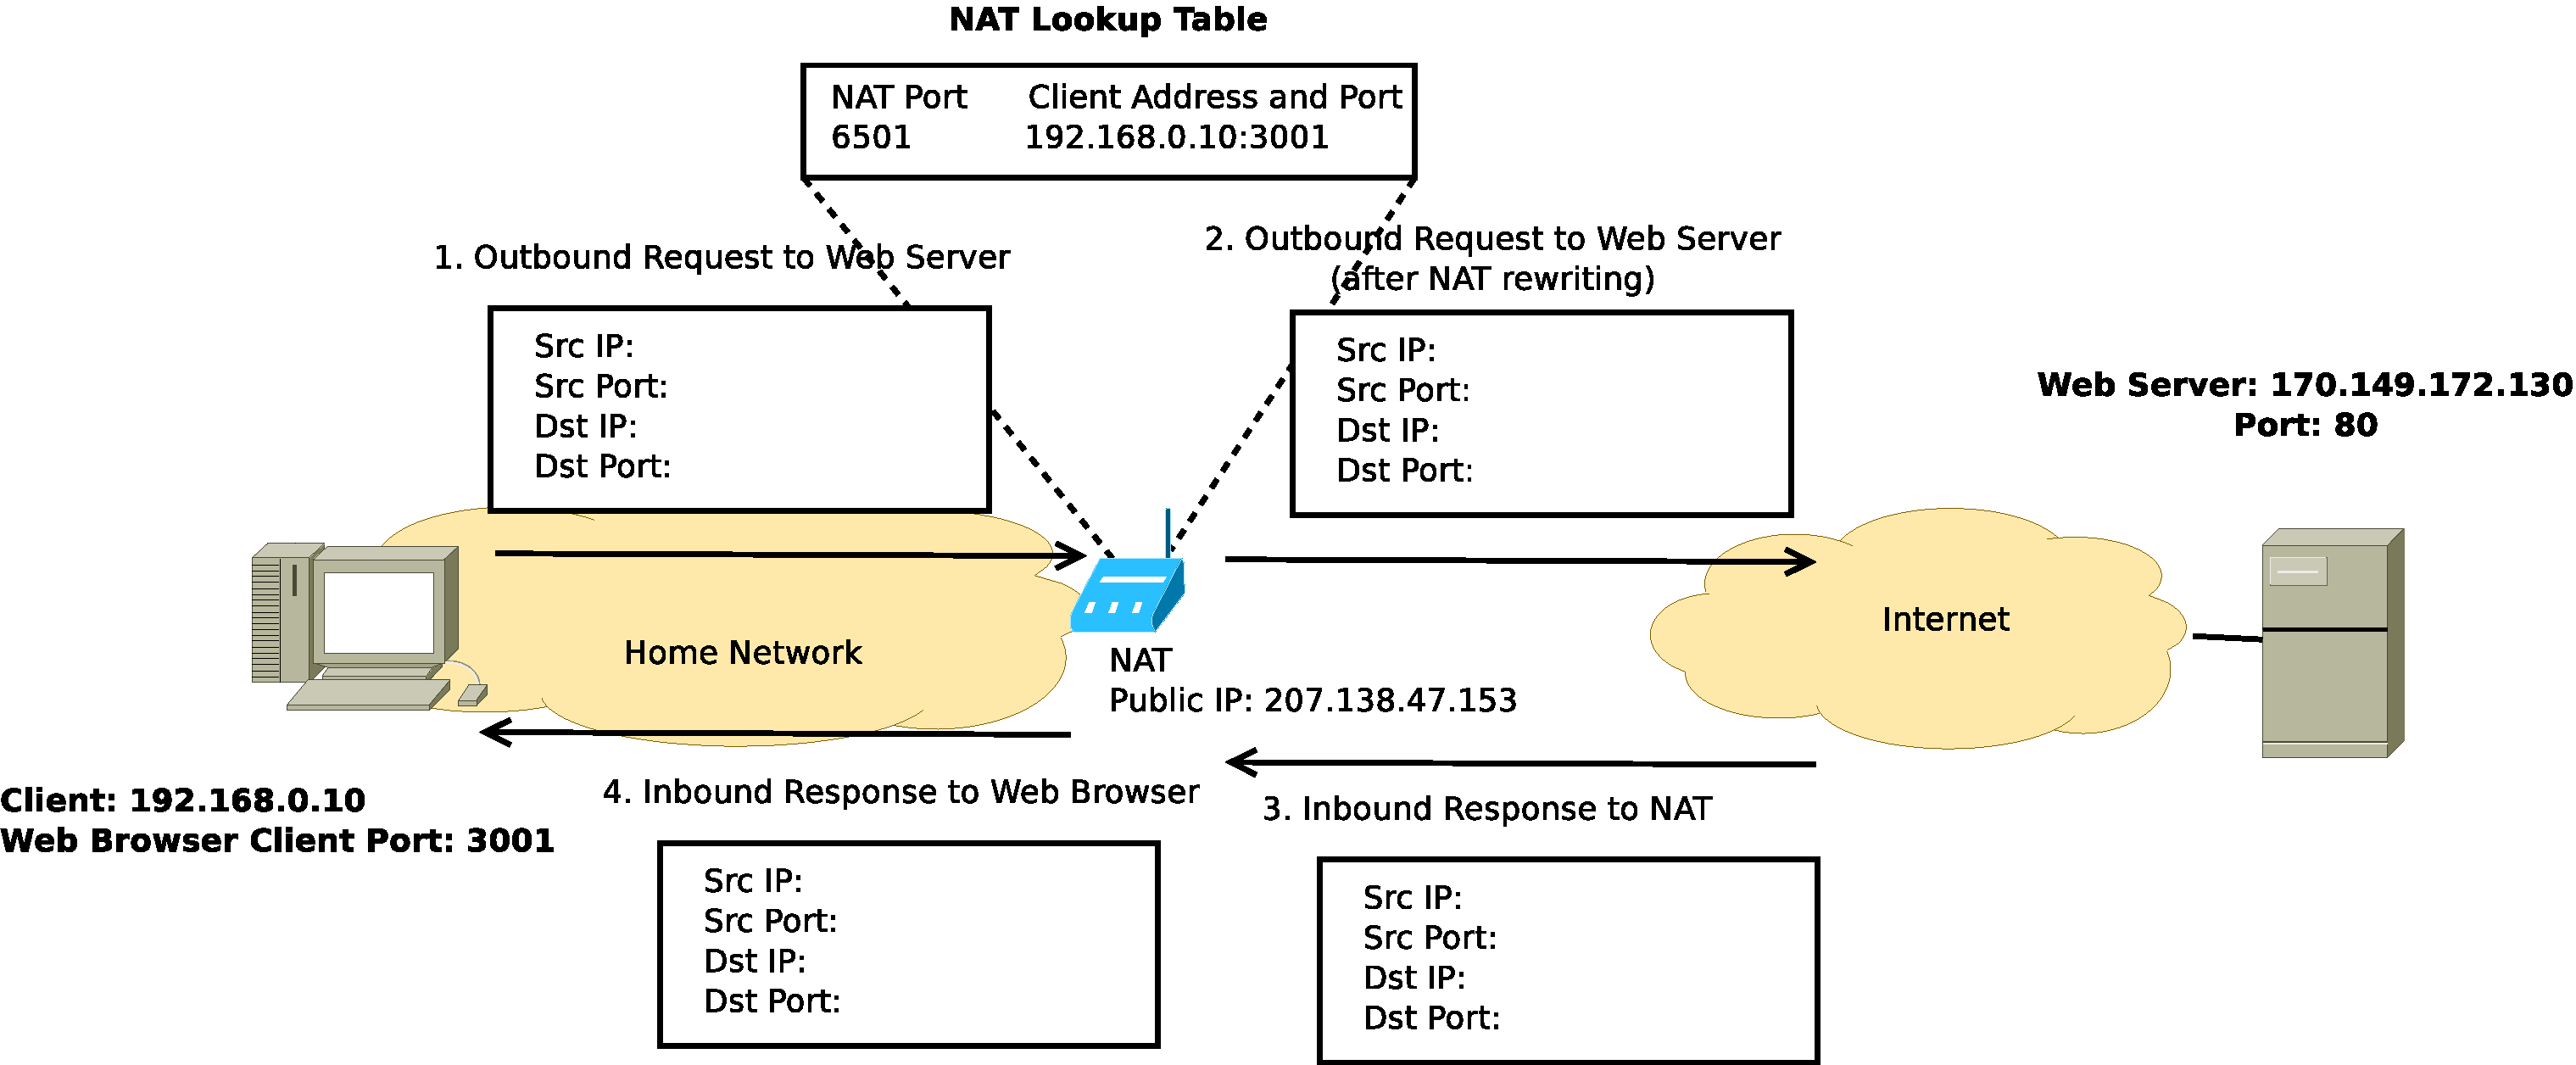
\includegraphics[width=1.2\linewidth]{home-nat}
\end{center}

\begin{itemize}
\item Briefly explain the why NAT devices need a lookup table, and how
  this lookup table would be populated.
\item Given the lookup table we provided, fill in the missing source and
  destination IP and port numbers on {\em all four packets} in the diagram above,
  when the client in the home attempts to send a packet to a Web server
  on the Internet.
\end{itemize}
% ~\ansbelow
\vspace{1.25in}
\eprob
\sols{
\vspace{-1.25in}
\begin{answer}
\end{answer}
}

\newpage
\section{TCP Congestion Control}

\prob{5} Suppose that, at a given time, a TCP sender has a congestion
window of 10 packets, that each packet is 1500 bytes, and that the
round-trip time between the sender and receiver is 100 milliseconds.
What throughput can the TCP sender achieve?  {\em Give your answer in
  bytes per second and show your work.}  \ansbelow \eprob
\vspace{1.25in}
\sols{
\begin{answer}
\end{answer}
}

\pagebreak
\prob{16} Consider the ``TCP sawtooth'' below, which shows the evolution
of the TCP congestion window size for a sender over time. Assuming this
TCP connection is using the usual additive incraese multiplicative
decrease (AIMD) congestion control algorithm. {\em You may need the back
  of a page to answer some of this question.  If you need more space,
  please indicate where we can find your answer, such as on the back of
  this page.}
\begin{center}
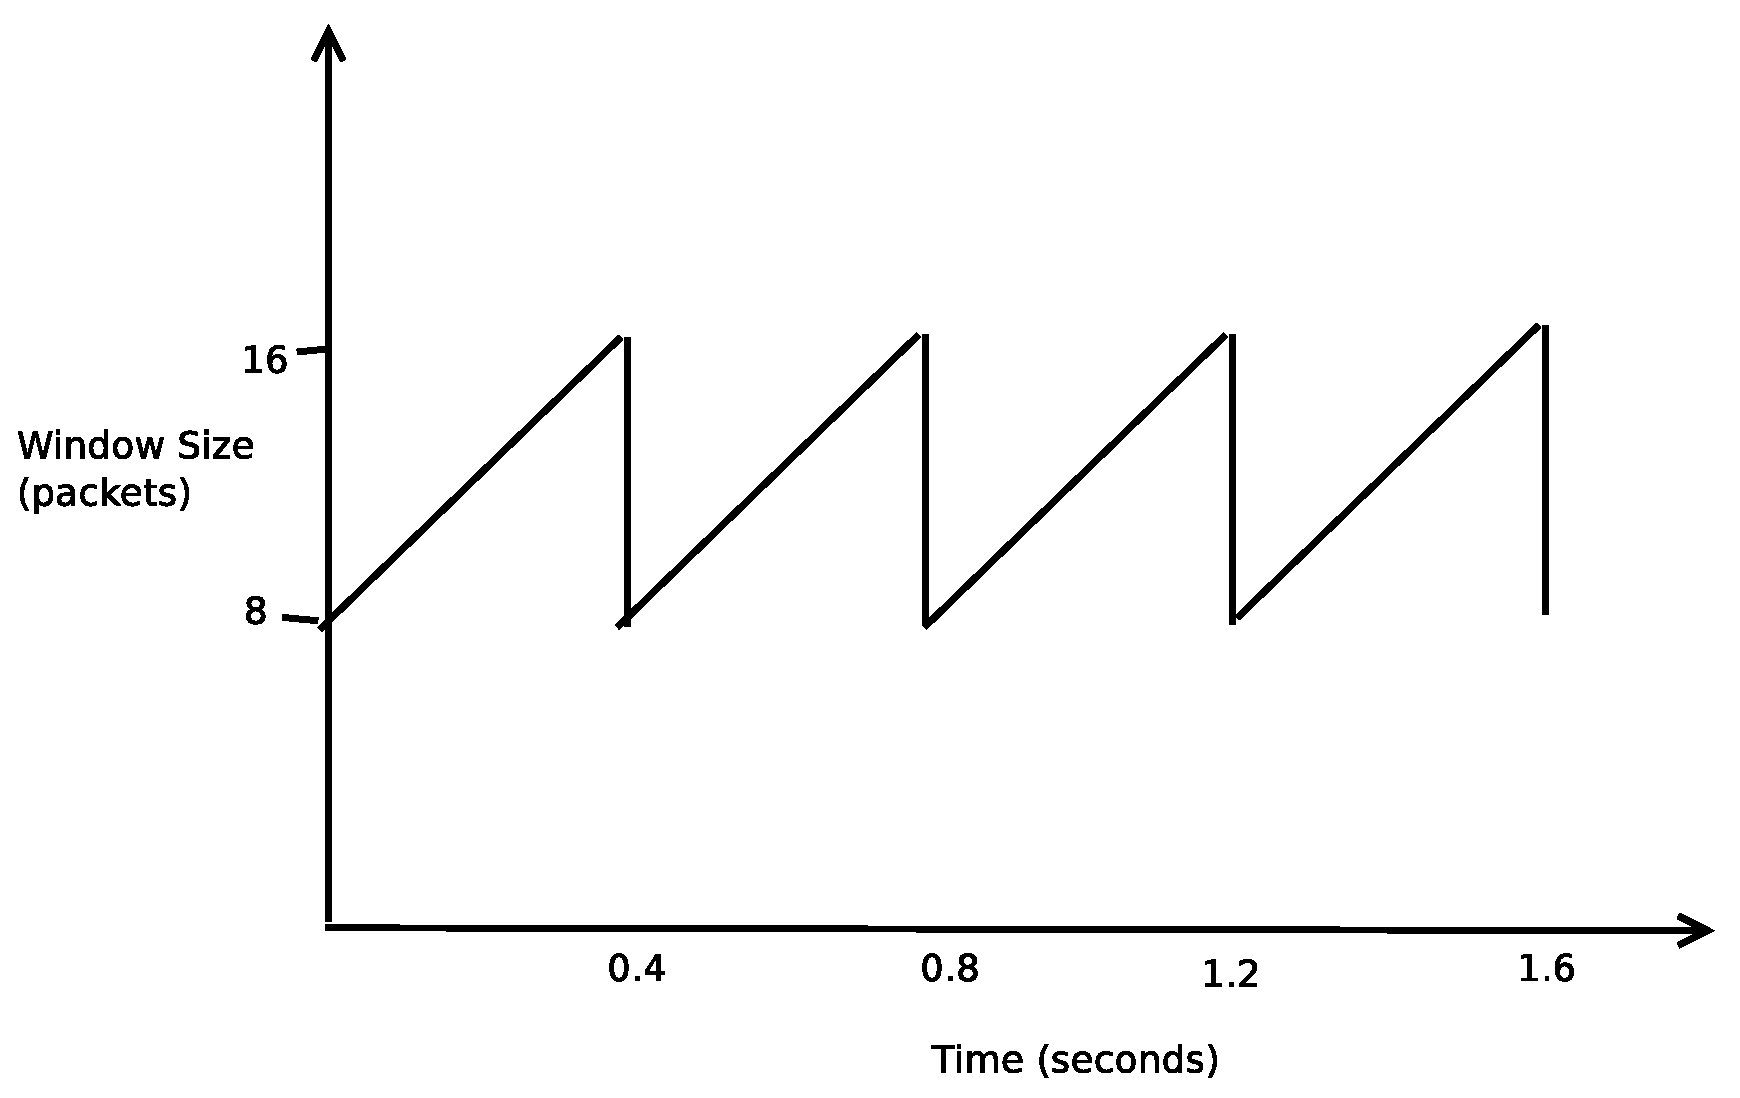
\includegraphics[width=0.65\linewidth]{tcp}
\end{center}
\begin{itemize}
\item[(a)] Draw arrows on the diagram where packet loss occurs.  Clearly
  label your arrows with the text ``packet loss'' so we know what you're
  pointing at. 
\item[(b)] What is the round trip time between the sender and receiver?
  Briefly show your work/explain your answer.
\item[(c)] Assuming {\em 1000-byte packets}, what is the average sending rate
  of the sender, in bytes per second?  (You can assume that the y-axis
  on the diagram is to scale, and you can give your answer either
  numerically or graphically.  If you can't compute the rates in bytes
  per second, give the average window size for partial credit.)
\item[(d)] Suppose that the data being sent over this connection is a video
  stream, and that the receiver wants to ensure ``smooth'' playout.
  What is the minimum amount of buffering that the client should have to
  ensure that the receiver can play out at the average rate, without
  interruption?  A numerical answer is better (show your work), but if
  you cannot figure out the math, you can give an answer graphically.
\end{itemize}
~\ansbelow \eprob
\vspace*{1.25in}
\sols{
\begin{answer}
\end{answer}
}



\newpage
\section{Web Performance and Caching}

\prob{4} Consider the Web page shown below.  Circle the parts of
the page that most likely can and should be cached on a local cache in a content
distribution network.  {\em Explain your answer.}  ~\ansbelow \eprob
\begin{center}
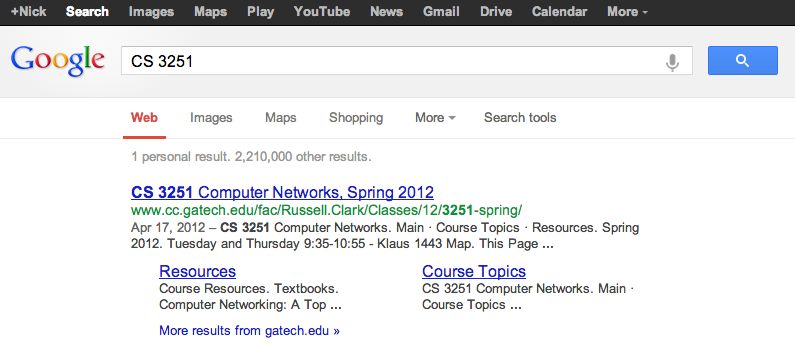
\includegraphics[width=\linewidth]{google-cs3251}
\end{center}
\vspace*{1.5in}


\sols{
\begin{answer}
\end{answer}
}

\prob{4} Suppose that a typical Web browser can open multiple TCP connections in
parallel {\em to each unique domain name}.  Describe how a Web site
designer might use the DNS to name Web objects so that such a client
browser might load the page more quickly.
~\ansbelow 
\eprob
\vspace*{1.25in}
\sols{
\begin{answer}
\end{answer}
}

\pagebreak
\prob{15} Consider the partial waterfall diagram below, for {\tt
  http://www.gatech.edu/}.  
\begin{center}
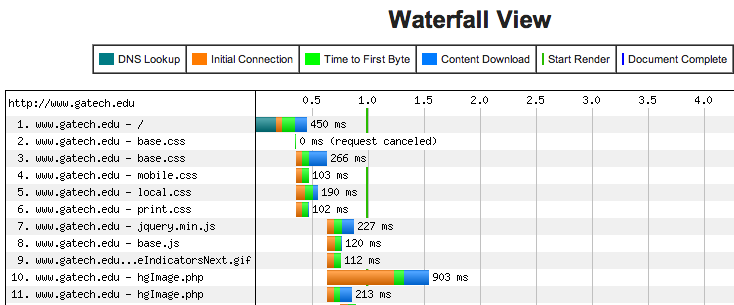
\includegraphics[width=\linewidth]{gt-waterfall}
\end{center}
\begin{itemize}
\item[(a)] How many TCP connections does this Web browser open in parallel?
\item[(b)] Which object downloads benefit from DNS caching? (You can use
  the object numbers in your answer to save writing.)
\item[(c)] Explain why persistent HTTP connections can reduce overall
  page load time, when they are used. Does the Georgia Tech site use
  persistent HTTP connections?  How can you tell?
\end{itemize}
 ~\ansbelow 
\eprob
\vspace*{1.25in}
\sols{
\begin{answer}
\end{answer}
}


\newpage
\section{Firewalls (+ Bonus Design Question)}

Suppose that Georgia Tech wants to only allow access to some of its Web
content for clients who are on campus.  (For example, Georgia Tech might
post a video stream that it wants to ensure is only visible on campus.)

To do so, it implements a stateless IP-based firewall that checks the
source IP address of the Web client making the HTTP request and sends a
TCP ``reset'' to any client whose source IP address is not inside of the
Georgia Tech network.

\prob{8} George Burdell is graduating next month and wants to continue
to be able to download this ``Georgia Tech only'' content, even after he
gets out.  He thinks that a carefully positioned Web proxy could help
him evade Georgia Tech's IP address-based filter.  Explain where George
should deploy his proxy, with respect to the client and the Web site,
and how the proxy could defeat the IP-based firewall.
~\ansbelow \eprob
\vspace*{1.25in}
\sols{
\begin{answer}
\end{answer}
}

\newpage
\prob{5} {\bf Bonus!! Optional!} The Georgia Tech Office of Information
Technology notes that you've completed CS~3251 and wants to hire you to
ensure that people like George can't continue to download ``GT only''
content, even in the presence of Web proxies.  Explain how you might
design a more sophisticated firewalling system to detect that client
requests like George are being sent through a proxy, as opposed to
originating directly from the client.
~\ansbelow \eprob
\vspace*{1.25in}
\sols{
\begin{answer}
\end{answer}
}





\newpage
\section*{Congrats! + Feedback + Thank You}
{\bf This page is anonymous.}  Rip this off from your exam, and turn it
in separately if you like.  You'll get five points for simply ripping
off the last page of the exam, but I'd prefer if you fill it out and
hand it in in a separate stack.

{\it Congratulations on finishing! Thank you for taking
this course with us.  We have really enjoyed the pleasure of teaching
it, and we have enjoyed your enthusiasm for the material.  We know that
not everything has been ``easy'', but we hope that now that the course
is over, you will walk away with some useful knowledge and experience
that you will use in the future, and will remember us fondly. :-)}

\vspace*{0.5in}

What was the best part of the course?  Anything is
fair game here (topics, course structure, board technique, etc.).
\vspace{0.5in}

What was the part of the course you'd like to see improved (or removed)?
\vspace{0.5in}

What was the best thing you learned in this course?
\vspace{0.5in}

What part of the course was not useful, in terms of your learning (if any)?
\vspace{0.5in}


In future offerings, what single thing would you recommend to improve
the course?
\vspace{0.5in}

Have you filled out CIOS?  If ``no'', please do it soon.  We will remind
you at the project demos. :-)




\label{lastpage}
\end{document}
